\documentclass[a4paper,11pt]{scrartcl}

\usepackage{biblatex}
\usepackage{lmodern}
\usepackage[T1]{fontenc}
\usepackage[a4paper, total={14cm, 24cm}]{geometry}
\usepackage{textcomp}
\usepackage{gensymb}
\usepackage{graphicx}
\usepackage{float}
\usepackage{caption}
\usepackage{hyperref}
\usepackage{paralist}
\usepackage{xcolor}
\usepackage{subcaption}
\usepackage[font={footnotesize,it}]{caption}
\usepackage{amsmath,amssymb,amsthm} 
\usepackage{url}
\usepackage{xspace}
\usepackage{algorithmic}
\usepackage{mathpazo}
\usepackage{booktabs}
\usepackage{subfiles}
\usepackage{silence}
\usepackage{listings}

% [Settings]

\WarningFilter{DuplicateLabels}

\newcommand{\ie}{ie}
\newcommand{\eg}{eg}
\newcommand{\reffig}[1]{Figure~\ref{#1}}
\newcommand{\refsec}[1]{Section~\ref{#1}}

\setcapindent{1em} %-- for captions of Figures
\setlength\parskip{1em plus 0.1em minus 0.2em}
\setlength\parindent{0pt}
\sffamily

\renewcommand{\algorithmicrequire}{\textbf{Input:}}
\renewcommand{\algorithmicensure}{\textbf{Output:}}

\addbibresource{ref.bib}
% [Title Page] (could be split away)

\titlehead{\centering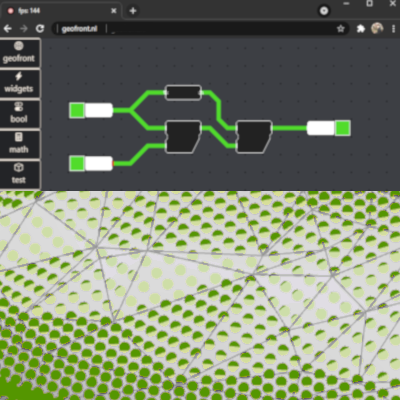
\includegraphics[width=12cm]{images/thumbnail.png}}
\title{Thesis Proposal: \\
Client-side geo-processing using WebAssembly and Visual Programming
}

\author{
  Jos Feenstra\\
  student \#4465768 \\
  \url{me@josfeenstra.nl}\\
  \\
  1st supervisor: Stelios Vitalis \\
  2nd supervisor: Ken Arroyo Ohori \\
}

\date{November, 2021}

\begin{document}

\clearpage\maketitle
\thispagestyle{empty}
\sffamily

\begin{center}
  \textbf{Key words:} Geomatics, WebAssembly, 3D geometry, Geo processing, Client side, Visual programming, 
\end{center}

% [Table of Content] 
\newpage
\tableofcontents

% [Body]
\newpage
%-------------------------------------------------------------------------------------------------%
% An introduction in which the relevance of the project and its place in the 
% context of geomatics is described, along with a clearly-defined problem statement.
% [KEN]
% instead, I think you can start by saying that web applications are popular
% explain the benefits briefly
% apart from having no installation

% then, I think you can make a better argument for your thesis overall
% explain that historically, thin client fat server was the standard
% for the reasons you listed
% and then directly explain why this is potentially changing now

\newpage
\section{Introduction}

% Dissolving the discrepancy between visualization \& processing in web-apps.

% web is popular 
% geoweb-applications are popular 
% online geodata processing is popular 
% client-side geodata processing 


% STELIOS: Relatively slow
 
% show an example 

Interactive, browser-based \ac{gis} applications form an indispensable component of the modern geospatial software landscape. A web application is cross-platform in nature, and offers ease of maintainability and access, since no installment or app-store interaction is required to update or run the app. The ability be placed as a supplement within the larger context of a webpage is also not trivial. These features have made the browser a popular host for many \ac{gis} applications, especially when targeting end-users. 

% streamline these three paragraphs.
% I want something like -> problem: limitations. 

Despite the popularity of \ac{gis} web applications, the range of actual \ac{gis} abilities these applications are capable of is very limited. For example, \ac{geoprocessing}, like CRS translations, interpolation, boolean operations, or raster transformation kernels are usually not present within the same software environment as the web app. This limited range of capabilities limits the usefulness of \ac{gis} web applications, and with it the number of use cases a \ac{gis} web application can serve. Current geospatial web applications serve for the most part only as lightweight viewers; visualizers of pre-processed data. If web applications gain these functionalities, they could grow to be just as diverse and useful as desktop \ac{gis} applications. It would allow for a new range of interactive web applications, in which data users can post-process geodata quickly, uniquely, and on demand.

This raises the question of Why. Why are web \ac{gis} applications limited to just be viewers?

% This raises the question: why is this not done yet? two reasons 
% 1. People are content with server-side geoprocessing 
%    -> BUT: this does not serve every use-case 
% 2. Client-side geoprocessing is hindered by javascript and the web environment
%    -> NOT ANYMORE: WebAssembly
% 
% 
% To solve 2: WebAssembly
% To solve 1: We offer a case study which demonstrates a unique type of application which would not be possible without client-side geoprocessing. 

However, by making the functionality of an application not self-contained but distributed, 

The improvements of client-side hardware have opened up a second possibility: client-side geoprocessing, directly within a web application. By doing this, the hard divide between client visualization and server processing could be bridged.  while at the same time driving down the operational costs of geoprocessing servers. This is why client-side \ac{geoprocessing} in web applications is slowly gaining traction during the last decade \cite{kulawiak_analysis_2019, panidi_hybrid_2015, hamilton_client-side_2014}. 

% Interactive geospatial data manipulation and online geospatial data processing techniques are described as "current highly valuable trends in evolution of the Web mapping and Web GIS" \cite{panidi_hybrid_2015}. 

However, serious drawbacks to client-side geoprocessing where encountered during these studies. Browser-based geoprocessing suffers from the fact that it will need to be written in the `JavaScript` programming language. Previous attempts at client-side geoprocessing have shown that JavaScript based geoprocessing libraries do not offer the performance required for proper geodata processing \cite{hamilton_client-side_2014}. 
Moreover, the JavaScript library ecosystem does not offer viable alternatives to industry-standard libraries like CGAL and GDAL. 
% This would require alternatives to be rewritten in JavaScript, or would require the source code of mature libraries to be compiled to JavaScript. Both these solutions would be difficult to maintain, and would still end 
% Both these solutions contain many imperfections. The first option would be an inefficient, time-consuming task, and would mean code duplication. 
% The second option would mean taking C++-based libraries such as CGAL, and compiling them to a special, fast subset of JavaScript called `asm.js` using the `emscripten` compiler \cite{zakai_emscripten_2011}. 
% While this is more fast and reliable, it contains its own set of problems. 
% The generated, rather large JavaScript files usually take a long time to download, to scan, and to be properly optimized by a JavaScript Just In Time (JIT) Compiler \cite{haas_bringing_2017}. 

An emergent technology poses a solution to both problems. At the end of 2019, the \ac{w3c} officially pronounced WebAssembly as the fourth programming language of the web \cite{w3c_world_2019}. Since then, all major browsers have added official WebAssembly support. \ac{wasm} is a binary compilation target meant to be small, fast, containerized, and platform \& source independent \cite{haas_bringing_2017}. \ac{wasm} surpasses javascript in almost all performance aspects: it loads quicker, it is scanned quicker, and since it is close to bytecode, it can often run at a speed comparable to system level programming languages like C++ and Rust \cite{jangda_not_2019}. 

% \cite{beilschmidt_vat_2017}


% Related studies concerned with the performance of WebAssembly, together with the existing software around WebAssembly, pose enough evidence to suggest  theoretically possible (SOURCE: Emscriptem). 
% However, this leaves the question whether it is practically possible unanswered, evident by the fact that no wasm-powered geoprocessing tools exists at the time of writing this study. 

\newpage

% stelios: Speed up 

\subsection{Problem}

If WebAssembly performs as described by \cite{haas_bringing_2017} and \cite{jangda_not_2019}, it could theoretically be the missing link to make client-side geoprocessing viable. However, no wasm-powered geoprocessing tools exists yet at the time of writing. Hypothetically, this is because of two reasons. Firstly, WebAssembly brings along many practical uncertainties:

\begin{itemize}
  \item Do geoprocessing libraries directly compile into WebAssembly? If not, which workarounds are needed? 
  \item Will a \ac{wagl} load efficiently, or should they be split up into parts, and loaded lazily? 
  \item How well do \ac{wagl} operations perform in a browser, compared to their native counterparts? What can be done to make this difference as small as possible?
\end{itemize}

Secondly, the way geoprocessing is supposed to be performed within the context of a web-browser remains unknown. The above list of implementation considerations cover only how \ac{wagl}'s can be \emph{run}. Potential answers do not indicate how \ac{wagl}'s can be \emph{used}. \cite{jangda_not_2019} warns against assessing WebAssembly in a vacuum, and notes how its performance is highly dependent on the way it is used, and the context in which it is used. This context of geoprocessing within a web-browser brings up many considerations as well: 

\begin{itemize}
  \item How will users upload or specify the input in a web-browser?
  \item Can the transformations offered by \ac{wagl}'s be used like functions? Or do they require special services, such as a wrapper library, virtual file system, or a virtual Command line interface? 
  \item How can users recieve and evaluate the output in a web-browser?
  \item How can a sequence of geoprocessing steps be chained together in a web-browser?
  \item How can a web-based \ac{ui} or \ac{gui} facilitate all these functionalities?
\end{itemize}

These two sets of unknowns are highly dependent upon each other. Together, they form a barrier preventing further development of client-side geoprocessing. Since no wasm-powered, client-side geoprocessing application exist yet, there is no way to answer these questions, and no way to confirm the theoretical benefits of WebAssembly for client-side geoprocessing, and the geospatial community at large.



\subsection{Use Case}
% mini methodolody??


in order to demonstrate 

visual programming language.




%-------------------------------------------------------------------------------------------------%
\newpage

%-------------------------------------------------------------------------------------------------%
\subsection{Research Questions}

This study intends to discover if contemporary web technologies can facilitate client-side geoprocessing by seeking an answer to the following question:  

\textit{How to \textbf{design and create} a browser-based GIS environment which can \textbf{effectively utilize} \textbf{existing geoprocessing libraries}, using only the \textbf{current state} of \textbf{standard client-side web technologies}?}

\subsubsection*{Explanation}

% The research question is written purposefully written in the "how well does X support Y question" shape. To unpack its components: 

- \textbf{design and create}: The wording 'design and create' is used to signal that this will consider the theoretical design , as well as the practicalities of creating this design. 

- \textbf{Standard client-side web technologies}: This phrase is meant to limit the scope to only the standard, core technologies of major browsers (Chrome, Edge, Safari, Firefox). This means the four languages \ac{wasm}, CSS, JavaScript and HTML. Additionally, HTML5 gives us WebGl, the 2d Canvas API, SVG's, and Web Components to work with.

- \textbf{Current state}: The study will use contemporary, even bleeding edge features of the modern web, but its findings will nonetheless be bound to this time of writing, as web technologies in particular quickly change. 

- \textbf{Existing geoprocessing libraries}. This wording expresses this studies desire to explore the usage of existing geoprocessing libraries, rather than to recreate geoprocessing libraries from scratch.

- \textbf{Effectively utilize}: The study intends to not only find out how \ac{wagl}'s can be \textit{run} in a browser, but also how \ac{wagl}'s can be \textit{used}. 


\subsubsection*{Sub Questions}

The following sub-research questions are needed in order to answer the main question. The methodology chapter will explain the choices of these sub-questions. 

\textit{1 : What is the most fitting methodology of compiling C++ geoprocessing libraries to WebAssembly?}

\textit{2 : How to design and create a client-side geoprocessing interface for data-users?}

\textit{3 : How can wasm-compiled geoprocessing libraries be distributed and used in a client-side geoprocessing interface?}

\textit{4 : What are the advantages and disadvantages of GIS applications created using a client-side geoprocessing environment powered by WebAssembly?}

\newpage
\subsubsection*{Assessment}

At the final conclusion of the proposed thesis, we can answer if the designed and created GIS environment can indeed effectively utilize these geo-libraries.
this will be answered by quantitative and qualitative means:

Quantity
\begin{itemize}
    \item Have all required features been implemented?
    \item Which libraries can be used?
    \item What are the load \& run times of these libraries, compared to native execution?
\end{itemize} 

Quality
\begin{itemize}
    \item Have all design goals been met?
    \item Can data users 'effectively' handle input, process and output?
    \item Can the load \& run times be regarded as acceptable to use? 
\end{itemize} 


% ----
\subsection{Scope}


\subsection*{Will Include}

The 'will include' scope is represented by the Methodology chapter. 

%-----------------------------------------------------------------------------%
\subsection*{Will not include}

\subsubsection*{Server-side or Native WebAssembly} % **Client-side WebAssembly Only**

This study will limit itself to the \emph{client-side} usage of WebAssembly. 
A powerful case can be made for \emph{server-side}, or native level usage of WebAssembly, especially in conjunction with a programming language such as Rust. 
Rust compiled to WebAssembly could, compared to using python, java or C++, make geoprocessing more maintainable and reliable, while at the same time ensuring memory safety, security, and performance \cite{clack_standardizing_2019}. 

Server-side or native wasm is beyond the scope of this paper, but would be an excellent starting point for future work. Note that this also means that research into \ac{wagl}'s is important for more than just client-side geoprocessing. All geoprocessing could benefit from it.



\subsubsection*{Web Processing Service} % Will not be dealing with WPS 

% offered as server-side geoprocessing services.  
Similarly, this study will exclude the OGC standard of the \ac{wps} \cite{ogc_web_2015}, since these services do not offer \emph{client} side geoprocessing, but instead offer \emph{server} side geoprocessing. A client-side application \textit{could} create an interface to use such a service, to essentially offer geoprocessing to clients, but this study regards a solution like that as a workaround, not a true solution to the problem of client-side geoprocessing. 

This is not to say that client-side geoprocessing replaces the need for \ac{wps}. 
future work could research the possibility of utilizing a hybrid strategy of both client-side and server-side geoprocessing, following in the footsteps of \cite{panidi_hybrid_2015}. 

% Still, We must briefly discuss the \ac{wps}, since it seems to offer a solution to the problems addressed.

%The OGC standard of the \ac{wps} offers a set of protocols to standardize geoprocessing on a server. By specifying input data and instructions to one of these services, polling the status of the process, and then downloading the results once finished, a user can process geodata on a server. If a client-side application creates an interface to use such a service, it can essentially offer client-side geoprocessing.

% While this is more like a workaround for client-side geoprocessing than a solution, it can nonetheless be preferred. A Web Processing Service is an excellent solution when client-side hardware is limited, and when server-side resources are abundant. It is also more efficient if the datasets required for geoprocessing are already located on these servers, and when working with geo-datasets too large to store locally. 

% situational cuts both ways 

% a \ac{wps} do not replace the need for client-side geoprocessing, for much of the same reasons a \ac{wps} does not replace the need for native \ac{gis} applications like QGIS or ArcGIS.  

% The usefulness of a \ac{wps} is, just like client-side geoprocessing, situational. 

% For much of the same reasons \ac{wps} does not replace the 


% reasoning from the perspective of client-side geoprocessing, a \ac{wps} does not offer a true solution to the problem of client-side geoprocessing, but only a workaround. 


% When the reverse is true however, and when the application needs to remain interactive and responsive, other solutions are required.

% While 

% Future work could research the possibility of utilizing a hybrid strategy of both client-side and server-side geoprocessing, following in the footsteps of \cite{panidi_hybrid_2015}. 


\subsubsection*{Usability Analysis} % 

While usability is a major component of this research, no claims will be made that the developed use-case is more usable to native GIS applications or geoprocessing methods. This research attempts to solve practical inhibitions in order to discover whether or not client-side is \emph{an} usable option. If it turns out that this method is viable technically, future research will be needed to definitively proof \emph{how} usable it is compared to all other existing methods.  

% This paper seeks to first close this gap, limiting itself to overcoming the technical and design boundaries in the pursuit of practical client-side geoprocessing.

Similarly, a survey analyzing how users experience client-side geoprocessing in comparison to native geoprocessing must also be left to subsequent research. While this would gain us tremendous insight, client-side geoprocessing is too new to make a balanced comparison. Native environments like GRASSGIS, QGIS, FME or ArcGIS simply have a twenty year lead in research and development. 

\newpage
%-------------------------------------------------------------------------------------------------%
% A related work section in which the relevant literature is presented and 
% linked to the project. 
% It should show that you clearly know the problem you plan to solve, 
% and that you master the related work. 
\newpage

\section{Related work}

This chapter offers background literature on the aforementioned topics, and will explain how this literature relates to the proposed study. three related topics are regarded: prior studies on WebAssembly, Prior studies on client-side geoprocessing, and prior studies on geoprocessing interfaces.


\subsection{WebAssembly \& Geoprocessing performance}

% Why are you writing this? 

On 5 December 2019, the \ac{w3c} officially pronounced WebAssembly as the fourth programming language of the web \cite{w3c_world_2019}. Philippe Le Hégaret, the \ac{w3c} Project Lead, writes “The arrival of WebAssembly expands the range of applications that can be achieved by simply using Open Web Platform technologies. In a world where machine learning and Artificial Intelligence become more and more common, it is important to enable high performance applications on the Web, without compromising the safety of the users,”. Since then, most major browsers have added WebAssembly support.

To the best of the author's knowledge, and as of writing this proposal, no papers explicitly links WebAssembly and Geodata processing. The original paper paper on \ac{wasm} does state \textit{3d data processing} as one of the examples for high performance web applications \cite{haas_bringing_2017}.. What's more, Google Earth uses WebAssembly as seen in \reffig{fig:google-earth} \cite{google_google_2020}. How it is used is unknown due to the engine being closed-source, but it is speculated that \ac{wasm} is used to access code written for the original C++-based desktop application.


\cite{jangda_not_2019, haas_bringing_2017}.

\begin{figure}[!tbp]
  \centering
  \begin{minipage}[b]{0.80\textwidth}
    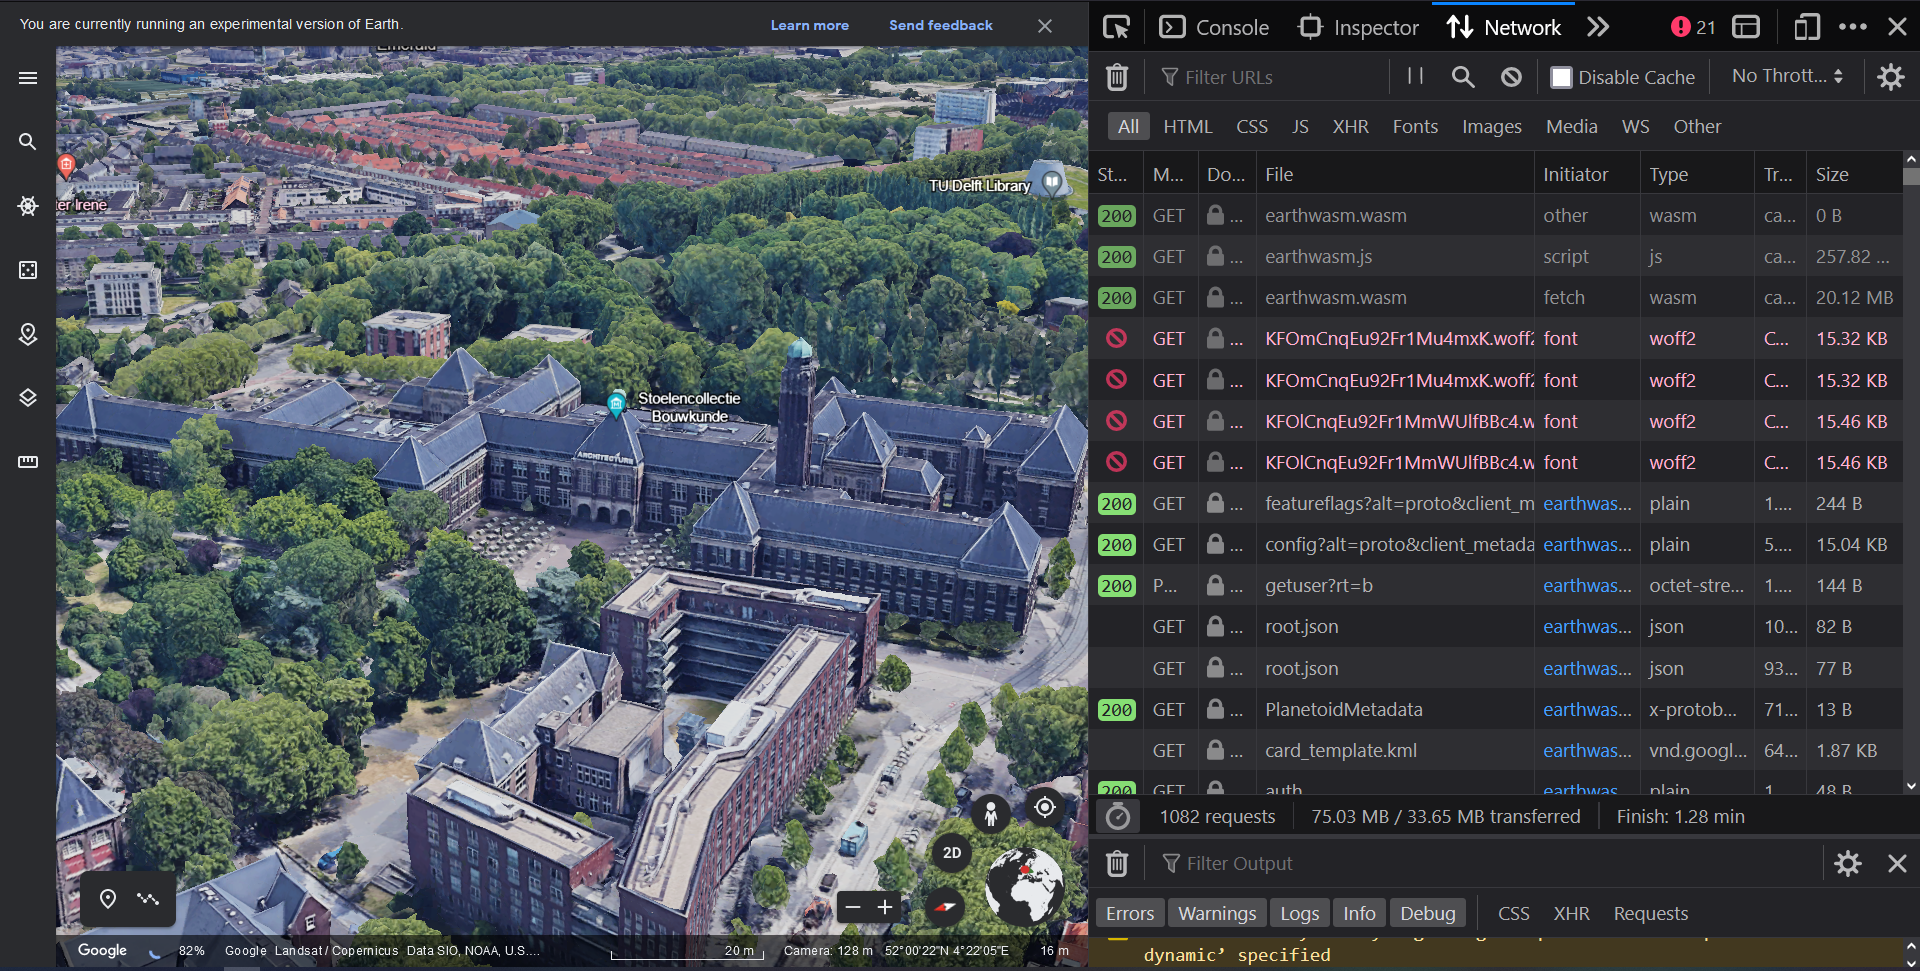
\includegraphics[width=\textwidth]{../images/google-earth-uses-webassembly.PNG}
    \caption{Google Earth utilizing WebAssembly. Source: \cite{google_google_2020}}
    \label{fig:google-earth}
  \end{minipage}
\end{figure}



The performance benefits of using WebAssembly for other purposes than geoprocessing have seen prior study. \cite{jangda_not_2019}.



% ORIGINAL PAPER

% ### x.x.x Bringing the Web up to Speed with WebAssembly
% This is the original paper introducing WebAssembly in 2017, co-written by software engineers from the major browser vendors Mozilla, Google, Apple and Microsoft. 
% It defines that a low-level compilation target should be
% save, fast, portable and compact.
% It continues by showing how previous attempts at low-level code on the web fail in at least one of these criteria, and that WebAssembly is the first to delivers on all of them. 
% The chapters following this up cover the design details of the language, and the decisions which had to be made to live up to the four criteria. 
% These details will become relevant when reasoning about why WebAssembly might be faster in one case versus another.
% <!-- proof of memory savety, proof of soundness  -->

% <!-- EXPLORE TYPES & EFFICIENT LOADING OF DATA TYPES BETWEEN UNRELATED LIBRARIES -->

% Chapter 6 and 7 also require special attention.
% Chapter 6 shows the possibilities available to a host environment for compiling, instantiating and invoking wasm binaries. 


% Chapter 7 : Implementation: 
% - validate
% - execution time
% - binary size 

% Initial benchmarks look promising
% large portion of benchmarks within 10% 

% <!-- 
% Interoperability It is possible to link multiple modules that
% have been created by different producers. However, as a low-
% level language, WebAssembly does not provide any built-in
% object model. It is up to producers to map their data types
% to numbers or the memory. This design provides maximum
% flexibility to producers, and unlike previous VMs, does not
% privilege any specific programming or object model while
% penalizing others. Though WebAssembly has a program-
% ming language shape, it is an abstraction over hardware, not
% over a programming language.
% Interested producers can define common ABIs on top of
% WebAssembly such that modules can interoperate in hetero-
% geneous applications. This separation of concerns is vital for
% making WebAssembly universal as a code format -->

%%%%%%%%%%%%%%%%%%%%%%%%%%%%%%%%%%%%%%%%%%%%%%%%%%%%%%%%%%%%%%%%%%%%%%%%%%%%%%%

% Not So Fast WebAssembly Paper 

% Paper exploring performance of WebAssembly more thorough.

% Starts out positive: current benchmarks (2019) are even better than those of the original paper (2017). 

% BUT 

% Those original papers cover a type of benchmark which uses mainly scientific operations as benchmarks. 
% Each of these operations are roughly 100 lines of code.
% This paper created a way to compile full, large-scale applications into WebAssembly, and proceeds to benchmark them. 
% They found that these types of applications run significantly slower and spikier.

% BUT 

% This might not be a problem for the scope of this research. 
% This research will deal with the originally criticized scientific purposes anyway.
% If it does turn out that wasm performs significantly slower the larger the binaries are, This research might explore disecting the C++ libraries into a number of tiny wasm Binaries, one per function for example, or per .cpp file. 
% As stated in the Wasm paper (SOURCE), it is possible to inject precompiled wasm binaries within other wasm binaries. 
% This way, the functionalities of one library could be lazy-initialized, so only the parts that are necessairy are being compiled and used. 
% Food for thought...

% ...

% A telling example of the cause of the loss in speed is this: 

% NATIVE: 
% C --{CLANG}-> x86-64 code

% WEB
% C --{EMSC}-> WASM --{JIT}-> x86-64 code 

% + Chapter 6 is very significant

% <!-- 6.4 Discussion
% It is worth asking if the performance issues identified here
% are fundamental. We believe that two of the identified is-
% sues are not: that is, they could be ameliorated by improved
% implementations. WebAssembly implementations today use
% register allocators (§6.1.2) and code generators (§6.2.1) that
% perform worse than Clang’s counterparts. However, an offline
% compiler like Clang can spend considerably more time to
% generate better code, whereas WebAssembly compilers must
% be fast enough to run online. Therefore, solutions adopted
% by other JITs, such as further optimizing hot code, are likely
% applicable here [19, 32].
% The four other issues that we have identified appear to
% USENIX Association 2019 USENIX Annual Technical Conference    117
% arise from the design constraints of WebAssembly: the stack
% overflow checks (§6.2.2), indirect call checks (§6.2.3), and
% reserved registers (§6.1.1) have a runtime cost and lead to in-
% creased code size (§6.3). Unfortunately, these checks are nec-
% essary for WebAssembly’s safety guarantees. A redesigned
% WebAssembly, with richer types for memory and function
% pointers [23], might be able to perform some of these checks
% at compile time, but that could complicate the implementa-
% tion of compilers that produce WebAssembly. Finally, a Web-
% Assembly implementation in a browser must interoperate with
% a high-performance JavaScript implementation, which may
% impose its own constraints. For example, current JavaScript
% implementations reserve a few registers for their own use,
% which increases register pressure on WebAssembly. -->

% <!-- 
% WHY PERFORMANCE LOST: LOST IN TRANSLATION 

% NATIVE: 
% C --{CLANG}-> x86-64 code

% WEB
% C --{EMSC}-> WASM --{JIT}-> x86-64 code 

% Seems to be

%  -->


% <!-- 

% TODO
% look into the specifics of the benchmarks provided 
% PolyBenchC seems to contain a lot of geometry operatinos, which seems good news for us



% SIGNIFICANT FOR GEOMATICS: 
% sync I/O is hard to do with webassembly. This could be detremental for many geomatics applciations



% The standard approach to running these applications today
% is to use Emscripten, a toolchain for compiling C and C++ to
% WebAssembly [39]. Unfortunately, Emscripten only supports
% the most trivial system calls and does not scale up to large-
% scale applications. For example, to enable applications to use
% synchronous I/O, the default Emscripten MEMFS filesystem
% loads the entire filesystem image into memory before the
% program begins executing. For SPEC, these files are too large
% to fit into memory

%  -->






\subsection{On client-side geoprocessing}

Client-side, browser based geoprocessing has seen academic interested throughout the last decade. 

- 

- timely nature

- performance 


% ### x.x.x 2014 Client-side versus Server-side Geoprocessing ...

% *These results demonstrated that the current implementation of web browsers are limited in their ability to execute JavaScript geoprocessing and not yet prepared to process data sizes larger than about 7,000 to 10,000 vertices before either prompting an unresponsive script warning in the browser or potentially losing the interest of the user.*

% This paper is very similar to what i'm doing, and it makes a conclusion that scared me at first glance. Then I saw that this is a paper out of 2014.

% The results of this paper are insightful, but do not directly applicable to this paper because of three reasons: 
% 1. The paper used javascript-based geoprocessing, not `asm.js` optimized. This is known to be inefficient. 
% 2. The paper stems from 2014. is before an incredible industry-wide performance increase of javascript interpreters. 
%    This is the result of technological development in the form of an arms race between the major browswer vendors. 
% 3. This paper will introduce WebAssembly to speed things up. 


%%%%%%%%%%%%%%%%%%%%%%%%%%%%%%%%%%%%%%%%%%%%%%%%%%%%%%%%%%%%%%%%%%%%%%%%%%%%%%%


% ### x.x.x Hybrid Geoprocessing Web Services

% This paper proposes a hybrid strategy, using the OGC Web Processing services as a starting point, and building client-side tools around it. This is different from the approach offered by this study, which starts from the well-known CGAL and GDAL geoprocessing libraries. The environment proposed by this thesis might offer OGC Web Processing services, inspired by this paper. 


%%%%%%%%%%%%%%%%%%%%%%%%%%%%%%%%%%%%%%%%%%%%%%%%%%%%%%%%%%%%%%%%%%%%%%%%%%%%%%%


% ### x.x.x Analysis of server-side and client-side Web-GIS data processing methods on the example of JTS and JSTS using open data from OSM and geoportal

% <!-- The last decade has seen a rapid evolution of processing, analysis and visualization of freely available geographic data using Open Source Web-GIS. In the beginning, Web-based Geographic Information Systems employed a thick-client approach which required installation of platform-specific browser plugins. Later on, research focus shifted to platform-independent thin client solutions in which data processing and analysis was performed by the server machine. More recently, however, the rapid development of computer hardware as well as software technologies such has HTML5 has enabled the creation of platform-independent thick clients which offer advanced GIS functionalities such as geoprocessing. This article aims to analyse the current state of Open Source technologies and publicly available geographic data sources in the context of creating cost-effective Web-GIS applications for integration and processing of spatial data. For this purpose the article discusses the availability and potential of Web-GIS architectures, software libraries and data sources. The analysis of freely available data sources includes a discussion of the quality and accuracy of crowd-sourced as well as public sector data, while the investigation of software libraries and architectures involves a comparison of server-side and client-side data processing performance under a set of real-world scenarios. The article concludes with a discussion of the choice of cost-effective Web-GIS architectures, software libraries and data sources in the context of the institution and environment of system deployment. -->

% This is a very relevant source




\subsection{On geoprocessing interfaces}

Finally, this proposal wishes to examine the state of the art of studies regarding geoprocessing interfaces. Unfortunately, most studies concerned specifically with geodata processing interfaces have a one to one relationship between application and interface. most papers do not state general user interface principles. At the same time, general UI studies are too broad, and while insightful, the scope is too big. 

Therefore, we stay close to home, and instead base interface considerations on

topic SDI research \& geoweb

interesting links can be made between

A noteworthy paper on this topic is Van den Brink's phd titled "Geospatial Data on the Web". Van den Brink states that geodata remains useful exclusively to experts in the field, despite all efforts to improve accessibility. 
She then presents the case for opening up geodata to a wider audience and more communities: "An important set of present-day users can be called “data users”: web developers, data journalists etc. who use different kinds of data, including geospatial data, directly to create applications or visualizations that supply information to end users (citizens). In order to achieve the wide re-use of geospatial data across communities, data should be easily accessible by these data users.". She also mentions the concept of FAIR geodata. Coined by \cite{mark_d_wilkinson_fair_2016}, The FAIR principles are a collection of four well-established assessment criteria used for judging the usability of data: Findable, Accessible, Interoperable, and Reusable. 

The proposed thesis acknowledges these concerns, and proposes to extend the concept of FAIR geodata to geoprocessing as well. This thesis therefore aims to make its proposed software as Findable, Accessible, Interoperable, and Reusable as possible. 

It is for these reasons that the topic of user interface will be part of this thesis. 

UI : as Findable, Accessible, Interoperable, and Reusable as possible. 

open, cross community, base on both web, w3c standards and OGC.

for these reasons, VPL chosen, so even non-programmers



- Ravi?

Lots of research has been done on the topic of VPL's, and their advantages and disadvantages. 
(I explicitly want to name the cognitive dimentions paper, it is very good and appropriate, and contains many suggestions for future VPL's)


% WebAssembly has the potential to improve all four of those criteria for software. If an application is published on the web without login requirements, makes it so there is no difference between Findability and Accessibility. As soon as it can be found, it can be accessed. 

% Additionally, \ac{wasm} is created explicitly to make software more \textit{Interoperable} and \textit{Reusable}.
% A ac{wasm} compiled library will work the same, wherever it is run. It is a manifestation of the  
% \textit{Write once, use anywhere} paradigm, not completely unrelated to the \textit{Collect once, use multiple times} paradigm, as both aim to minimize redundancy.



%%%%%%%%%%%%%%%%%%%%%%%%%%%%%%%%%%%%%%%%%%%%%%%%%%%%%%%%%%%%%%%%%%%%%%%%%%%%%%%


To the best of the author's knowledge, no papers exist coupling VPL to geoprocessing.

Still, this is being done, evident by...


Examination of multiple VPLS:






\subsection{Conclusion}

- Time is important 
- 'missing link'



\newpage
%-------------------------------------------------------------------------------------------------%
% [HUGO]: The research questions are clearly defined, along with the scope (ie what you will not be doing).
% To help you define a "good" research question, 
% read \url{https://sites.duke.edu/urgws/files/2014/02/Research-Questions_WS-handout.pdf}.
% [ From Hugo's handout: ]
% 
% clear | focussed | unique | 
% start asking open-ended “How?” “What?” and Why?” questions. 
% Then evaluate possible responses to those questions
% While a good research question allows the writer to take an arguable position, 
% it DOES NOT leave room for ambiguity.
% 
% 1)Is the research question something I/others care about? Is it arguable?
% 2)Is the research question a new spin on an old idea, or does it solve a problem?
% 3)Is it too broad or too narrow?
% 4)Is the research question researchable within the given time frame and location?
% 5)What information is needed?
% 
% are you trying to accomplish one of these goals? 
% 1) Define or measure a specific fact or gather facts about a specific phenomenon. -> YES. IT TRIES TO GATHER FACTS ABOUT WEBASSEMBLY
% 4) Prove that a certain method is more effective than other methods. -> ONLY WASM compared to native
% Moreover, the research question should address what the variables of the experiment are, their relationship, 
% and state something about the testing ofthose relationships. 
% 
% [JF] : I really know what I want to do, and I am convinced improving the usability of geoprocessing tools is both valuable and Good. 
% 
\newpage
\section{This Study}

% This paper's main objective is to judge the fitness of WebAssembly for client-side geo-processing purposes. 
% This fitness will be judged quantitatively by means of performance benchmarks and compilation performance, as well as qualitatively by documenting the creation of a web-based geoprocessing application using WebAssembl
% The study aims to provide a guide for using WebAssembly for Geoprocessing


% ### This Study

% The aim of this study is to provide an environment meant for client-side geoprocessing using WebAssembly. This environment will be used to demonstrate if and how wasm-based, client-side geoprocessing is possible. At the same time, by presenting this environment, the study aims to explore the design possibilities of a web-GIS application equipped with such tools. 

% This will require research into the technical effectiveness of WebAssembly. C++ geoprocessing libraries such as CGAL & GDAL will be tested on their ability to be compiled, loaded, and used from a browser. This is compared against their compilation by other means, such as native binaries or the aforementioned `asm.js`. This research is complemented by an extensive 'case study' to explore the design possibilities of a web-application equipped with client-side geoprocessing. A thick-client web application will be created, and this will serve as platform for testing the aforementioned `wagl`'s. The tool and can be additionally used for acquiring, visualizing, and saving geodata. 





% "Can WebAssembly offer the performance and interoperablility with C++ needed for geoprocessing?"
% Can the "web ui", consisting of HTML, css and javascript, offer us enough to work with to create a UI needed for proper geoprocessing?% 

The studies main objective is to make geoprocessing more sharable, accessible and insightful by using the web. It does this by researching if the current state of client web technologies are ready for geoprocessing.
% This study's main objective is to determine if and how WebAssembly can practically enable client-side geoprocessing. 
It aims to gather facts and develop tools around both these technologies and client-side geoprocessing, so that this judgement can be fairly made. 
% 1 & 3
The required facts will be gathered by means of performance benchmarks, a compilation method comparison, and a distribution method comparison.  
% 2
The tools take the shape of a client-side GIS application using WebAssembly.
To ensure that these facts \& tools are unambiguous, reproducible, and re-usable, the study will offer guides on exactly how certain C++ geoprocessing libraries are converted to wasm. For the same reasons, it also presents implementation details and considerations of the geoprocessing environment.  
% 4
Finally, by presenting and using this environment, the study aims to explore the advantages and disadvantages of a client-side-GIS application equipped with native-level geoprocessing tools. 

% This will require research into the technical effectiveness of WebAssembly. 
% C++ geoprocessing libraries such as CGAL \& GDAL will be tested on their ability to be compiled, loaded, and used from a browser. 
% This is compared against their compilation by other means, such as native binaries or the aforementioned `asm.js`. 

% This research is complemented by an extensive 'case study' to explore the design possibilities of a web-application equipped with client-side geoprocessing. 
% A thick-client web application will be created, and this will serve as platform for testing the aforementioned `wagl`'s. 
% The tool and can be additionally used for acquiring, visualizing, and saving geodata. 

% (WebAssembly geoprocessing libraries -> `wagl`'s)

%-------------------------------------------------------------------------------------------------%
\subsection{Research Question}

\textit{How to \textbf{design and create} a GIS environment which can \textbf{effectively utilize} \textbf{existing geoprocessing libraries} within a web browser, using only the \textbf{current state} of \textbf{standard client-side web technologies}?}

% "How well can the \textbf{current state} of \textbf{standard client-side web technologies} make \textbf{existing geoprocessing libraries} \textbf{usable} in a browser?"

\subsubsection*{Explanation}

% The research question is written purposefully written in the "how well does X support Y question" shape. To unpack its components: 

- \textbf{design and create}: The wording 'design and create' is used to signal that this will cover both how this environment could theoretically be designed

- \textbf{Current state}: Note how the Related works section named (SOURCE)'s paper outdated, even though it was written in 2016. This is why this study will also be very timely. It will use contemporary, even bleeding edge features, but its findings will nonetheless be bound to this time of writing, as web technologies can quickly change in the future. 

- \textbf{Standard client-side web technologies}: This phrase is meant in a first principles sense: Examine the raw, core technologies the major browsers (Chrome (Edge), Safari, Firefox) offer without plugins or libraries. This study will cover: CSS, JS, HTML5, the DOM, WebGl, the 2d Canvas API, SVG's, and, its most recent addition, WebAssembly. 

- \textbf{Existing geoprocessing libraries}. This wording expresses this studies desire to explore the usage of existing geoprocessing libraries, rather than to recreate geoprocessing libraries from scratch.

- \textbf{Effectively utilize}: The study intends to not only find out how the geo-libs can be \textit{run} in a browser, but also how geo-libs can be \textit{used}. So besides covering qualities like performance and loading times, we will also be asking questions like: \textit{how do we specify the input?}, \textit{how do we recieve and evaluate the output?} and \textit{how can multiple steps be chained together?}, which is a vital component of geoprocessing. To seek answers to these questions, the study will regard questions of this nature as \textit{Interface} questions, and will explore the creation of a geoprocessing interface. 

\subsubsection*{At the conclusion}

At the final conclusion of the proposed thesis, we will answer if the designed and created GIS environment can indeed effectively utilize these geo-libraries.
this will be answered by quantitative and qualitative means:

Quantity
\begin{itemize}
    \item Have all required features been implemented?
    \item Which libraries can be used?
    \item What are the load \& run times of these libraries, compared to native?
\end{itemize} 

Quality
\begin{itemize}
    \item Have all design goals been met?
    \item Can users 'effectively' handle input, process and output?
    \item Can the load \& run times be regarded as acceptable? 
\end{itemize} 

% this can also be answered by qualitative means:
% - 
% - 
% - 

\subsubsection*{Sub Questions}

The following sub-research questions are needed in order to answer the main question. The upcoming methodology chapter will further explain the choices of these sub-questions. 

\textit{1 : What is the most fitting methodology of compiling C++ geoprocessing libraries to WebAssembly?}

\textit{2 : How to design and create a client-side geoprocessing interface?}

\textit{3 : How can wasm-compiled geoprocessing libraries be distributed and used in a client-side geoprocessing interface?}

\textit{4 : What are the advantages and disadvantages of GIS applications created using a client-side geoprocessing environment powered by WebAssembly?}

% ----
\newpage
\subsection{Scope}


\subsection*{Will Include}

The 'will include' scope is also represented by the Methodology chapter. 

%-----------------------------------------------------------------------------%
\subsection*{Will not include}

\subsubsection*{Server-side WebAssembly} % **Client-side WebAssembly Only**

This study will limit itself to the **client-side** usage of WebAssembly. 
A powerful case can be made for **server-side** usage of WebAssembly, especially in conjunction with a programming language such as Rust. 
Rust compiled to WebAssembly could, compared to using python, java or C++, make geoprocessing more maintainable and reliable, while at the same time ensuring memory safety, security, and performance [SOURCE: wasi, wasm-ai]. 
Server-side wasm is beyond the scope of this paper, but would be an excellent starting point for future work. 

Note that this also means that research into `wagl`'s is important for more than just client-side geoprocessing. All geoprocessing could benefit from it.



\subsubsection*{Web Processing Services} % Will not be dealing with WPS 

This research will exclude the OGC standard of web processing services (SOURCE), since these services are not about \emph{client} side geoprocessing, but instead cover \emph{server} side geoprocessing. 
Future work could, however, research the possibility of utilizing a vpl for WPS orchestration. 



\subsubsection*{Usability Analysis} % 

While usability is a primary motivation for conducting this research, no claims will be made that the developed geoprocessing environment is more usable to native GIS applications or geoprocessing methods. This research attempts to solve practical inhibitions in order to discover whether or not client-side is \textbf{an} usable option. If it turns out that this method is viable technically, future research will be needed to definitively proof \textbf{how} usable it is compared to all other existing methods.  

% This paper seeks to first close this gap, limiting itself to overcoming the technical and design boundaries in the pursuit of practical client-side geoprocessing.

Similarly, a survey analyzing how users experience client-side geoprocessing in comparison to native geoprocessing must also be left to subsequent research. While this would gain us tremendous insight, client-side geoprocessing is too new to make a balanced comparison. Native environments like GRASSGIS, QGIS, FME or Esri simply have a 20+ year lead in research and development. 

\newpage


\section{Preliminary Work}

Several projects have been carried out to prepare for this study. 

\subsection*{Research Assignment}

Geomatics small scale research assignment.
Testing out wasm for a geomatics web application.
Familiarizing with technologies.
Hybrid setup.

\subsection*{Prototype}

Nodes 

Geon engine


\subsection*{Internship}

Internship vaguely related
case for thick-client architecture

\newpage
%%%%%%%%%%%%%%%%%%%%%%%%%%%%%%%%%%%%%%%%%%%%%%%%%%%%%%%%%%%%%%%%%%%%%%%%%%%%%%%
% Overview of the methodology to be used.
% \newpage

\section{Methodology}

% <img src="../../../proposal/schemas/methodology/method.svg">

The study described by this proposal will be sizable, as well as complex. 
It contains many interlinked and interdependent components. 
As such, this study applies an incremental methodology with clear phases and in-between products, as a means of quality control while the study is carried out. 
It also eases the development process, as well as ensures sufficient results in the case the full scope of this study might become unfeasible. 

The five phases, based on the five sub-questions, are 1. Compile, 2. Develop, 3. Synthesize, 4. Benchmark, and 5. Utilize. Every phase will be concluded by an answer to its corresponding research question. See \reffig{fig:method} for a complete overview. As the figure suggests, Phase 1 and 2 can be executed in parallel, as well as phases 4 and 5. However, for the sake of clarity, this will be avoided. 

\begin{figure}
    \centering
    \graphicspath{ {../schemas/methodology/} }
    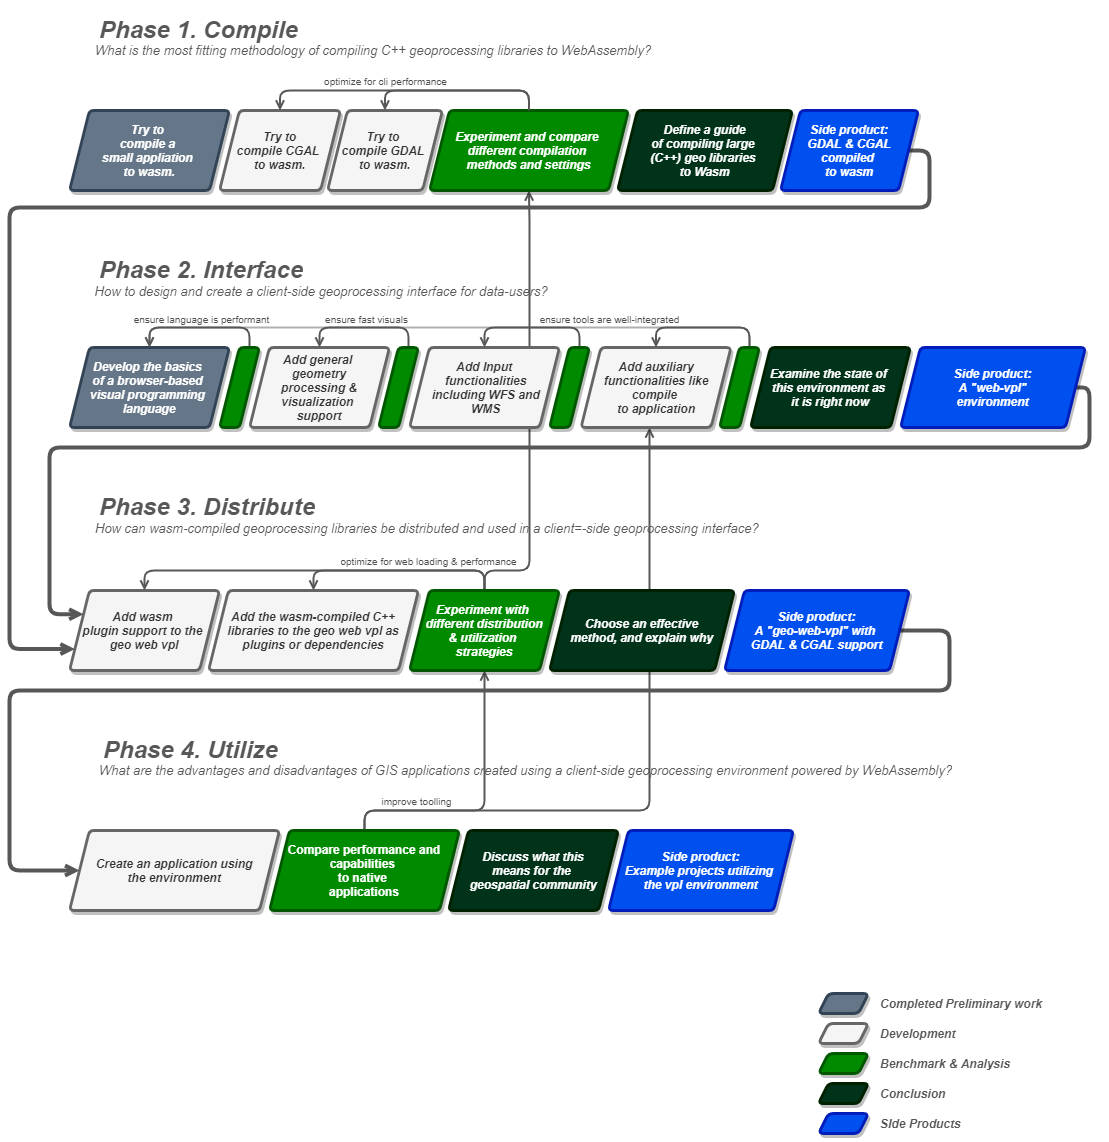
\includegraphics[width=14cm]{method.png}
    \caption{Methodology schema}
    \label{fig:method}
\end{figure}


\subsection{Phase 1: Compile}

The first phase will be about the procedure to successfully compile CGAL and GDAL to WebAssembly.

This will require research into the technicalities of the compilation target, as well as the compilation tool Emscripten (SOURCE).

The first phase will contrive of a number of steps:

- 1.1. Compile a small geoprocessing C++ script to wasm.
- 1.2  Compile CGAL \& GDAL to wasm.
- 1.3  Comparison and discussion of multiple wasm compilation methods and considerations for large libraries.


(mention preliminary work with hugo, and the knowledge gained by using WebAssembly)


\subsection{Phase 2: Develop}

% The second phase is the development of the aforementioned web-based geoprocessing tools. 

% The current plan is to shape this like a visual programming language. 

The second phase is characterized by the creation of a client-side geoprocessing environment. While all phases will entail some level of software development, this is the phase where an entire application will have to be created.

Just like the entire project, the development trajectory during phase 2 will be done incrementally, ensuring results can be produced and shown during all steps of the development. 

Creating a client-side geoprocessing application comes with many design considerations. 



Phase 2. Develop. ** a browser-based visual programming language (web-vpl), which can visualize geometry, and contains basic GIS functionalities.  


To provide an environment meant for client-side geoprocessing using WebAssembly,



A thick-client web application will be created, and this will serve as platform for testing the aforementioned ‘wagl‘’s. The tool and can be additionally used for acquiring, visualizing, and saving geodata.

At the end of this step, This environment will be usable 

basic mathematical and geometry procedures. 

and will not contain any geodata processing capabilities, nor WebAssembly. 





(mention preliminary work)

- 2D Canvas API / SVG 

- DAG : Directed Acyclic Graph

- Granular classes



\subsection{Phase 3: Synthesize}

Phase 3. Synthesize. **Combine** wasm to the environment to use the wasm-compiled CGAL and GDAL libraries.

in terms of distributing, loading, and using 
What is the optimal way of distributing, loading, and using?

hypothesis: splitting large C++ libraries up in smaller, maybe even "per function" compilation targets. 
Utilize WebAssemblies ability to accept dependencies.
Need to research more into Emscripten's capabilities.

\subsection{Phase 4: Benchmark}

The fourth phase will be a benchmarking phase. This is one of the later phases, to make use of the fact that an entire geoprocessing environment will have been created at this stage,which can then be used as a benchmarking test suite. 

The most important benchmarks that will have to be made is the comparison of the CGAL \& GDAL libraries natively versus fully integrated in the environment. Additionally, many "in-between" version are possible, which might pose valuable insight. In total, per method or functionality, five different states are of interest to this study:

\begin{itemize}
    \item Compiled and run as native binary (g++),
    \item Compiled to asm.js, run natively (node.js),
    \item Compiled to asm.js, run in a browser.
    \item Compiled to wasm, run natively (WASI),
    \item Compiled to wasm, run in a browser,
\end{itemize}



\subsection{Phase 5: Utilize}

Finally, When the VPL contains all tools necessary to be used to properly process geodata, a final assessment can be made by actually using the environment to create applications.
I hypothesize that applications equipped with client-side geoprocessing open up a whole range of new possibilities for both academic \& commercial benefits. 
I intent to discuss these aspects of the study during this phase. 



% Three different applications will be created using regular means (jupyter notebook, python, % panda's, etc)
% and these same applications will be created using the prototype web-VPL. 
% These two methods will then be compared on usability aspects and performance.   

% ## 5.3 Case Study

% > ### *Demo Application: On Demand Triangulator + Isocurves* 
% > 
% > ### Input: 
% > - Point Cloud
% > 
% > ### Output
% > - Line Curves / .png render of line curves
% > 
% > ### Steps: 
% > - Load ahn3 point-cloud (WFS Input Widget | WFS Preview Widget)
% > - Visualize point cloud on top of base map of the netherlands (WMS Input Widget | WMS > Preview Widget)
% > - Only select terrain points (list filter Operation)
% > - Construct a 2d polygon by clicking points on a map (Polygon Input Widget)
% > - Select Area of interest using a 2d polygon (Boundary Include Operation)
% > - Triangulate point cloud with a certain resolution (Triangulate Operation)
% > - Intersect the mesh surface with a series of planes (Isocurves from Mesh Operation)
% > - Preview data (MultiLine Preview Widget)
% > - Export data (MultiLine export Widget)
\newpage
%-------------------------------------------------------------------------------------------------%
% Having a Gantt chart is probably a better idea then just a list.
\newpage
\section{Planning and Organization}

This study 



A Gantt chart (FIGURE X) explains this planning more thouroughly
\newpage
%-------------------------------------------------------------------------------------------------%
% Since specific data and tools have to be used, it’s good to present these concretely, 
% so that the mentors know that you have a grasp of all aspects of the project.
\newpage
\section{Tools and data}

\subsection{Tools}
In order to perform the study this paper describes, several tools are needed. All tools mentioned are free and open source.

\subsubsection*{Typescript}
Typescript will be the programming language used for creating the main visual programming language application. Typescript is chosen over plain javascript, since the safeguards and type checks provided at compile time are very useful, especially when creating medium to large scale applications. 

Depending on the size of the application, a framework such as React or Vue might be used to offer structure.

\subsubsection*{HTML5}
HTML5 provides adequate features in order to create the actual GUI. Buttons and panels can be created using just HTML. The Canvas 2d API is an excellent method of drawing 2d shapes, and can be used to draw the components and cables of the VPL itself. Alternatively, this can also be done using Scalable Vector Graphics (SVG's). 

\subsubsection*{WebGl}
WebGl allows for performant web visualizations using syntax similar to OpenGL. This will be used to make preview visualizations of 2D and 3D data. Modern web browsers are equipped with WebGl by default. 

\subsubsection*{WebAssembly}
WebAssembly binaries, and its surrounding tooling, will of course be used. Modern browsers provide WebAssembly support by default. For running WebAssembly files locally, WASI, a native WebAssembly Runtime will be utilized. 

\subsubsection*{C++ \& Emscriptem}
Most geoprocessing libraries commonly used within the geospatial community are C++ based libraries, such as CGAL \& GDAL. A tool called Emscripten will be used to compile these libraries into WebAssembly. Additional C++ wrapper libraries might be written if direct compilation proves to be difficult. 

\subsubsection*{Rust \& wasm-pack}
Rust is the community preference for developing programs targeting wasm. 
The rust ecosystem contains a number of powerful tools such as wasm-pack, and the standard rust compiler includes wasm as a compilation target by default. If during this study a need arises for newly written geoprocessing libraries, Rust will be preferred over C++ for these reasons. But, by default, Rust will not be used during this study, since no well-known geoprocessing libraries exist within its ecosystem.

\subsection{Data}
This study is not dependent on specific datasets. However, in order to use Geodata processing libraries, we will have need of some data to start with. Demo data of the netherlands will be used, using the WFS and WMS services provided by the Dutch geodata portal PDOK. 


% [Appendix]
\newpage
\printbibliography

\end{document}